\section{Solution Cisco/AnyConnect}
La solution Cisco diffère des autres solutions, car l'ASA\footnote{Adaptive Security Appliance} a des fonctions plus limitées.
Il n'offre que deux VLAN avec la licence de base.

\subsection{Schéma de l'infrastructure}
L'ASA fait office de pare-feu et de passerelle SSL.
Comme chaque interface doit appartenir à un VLAN, l'un des VLAN est la zone \textit{outside} et l'autre est la zone \textit{inside}.
La zone \textit{outside} fait référence au réseau du laboratoire et l'\textit{inside} est mon domaine.
Dans ce cas-ci, les ordinateurs et les serveurs ne sont plus dans des zones distinctes (voir Fig.p.).
%\begin{figure}[ht]
%	\centering
%	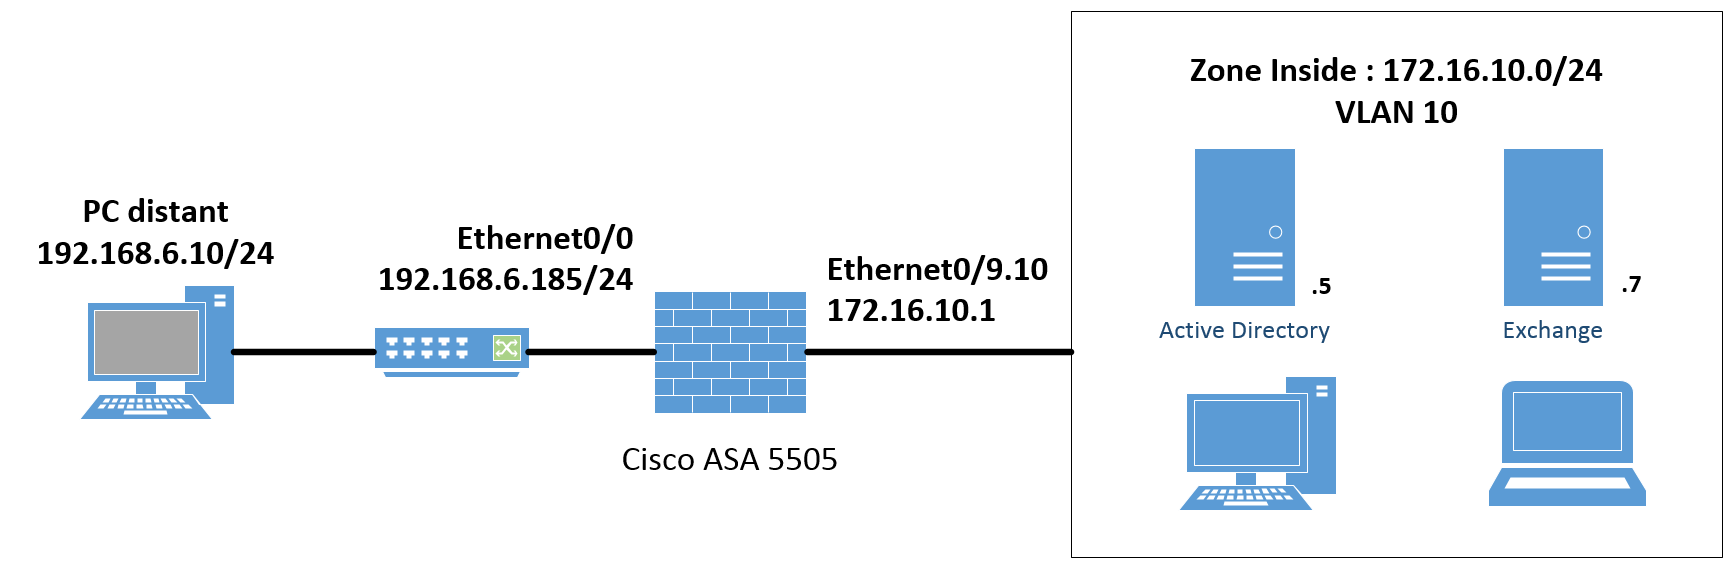
\includegraphics[width=16cm]{Cisco/schema.png}
%	\caption{Adressage des interfaces}
%	\label{fig:schemaCisco}
%\end{figure}
Pour l'adressage, j'ai conservé le même plan sauf que mon ordinateur interne se retrouve avec une adresse 172.16.10.0/24 (voir Fig.\ref{fig:ifCisco} p.\pageref{fig:ifCisco}).
\begin{figure}[ht]
	\centering
	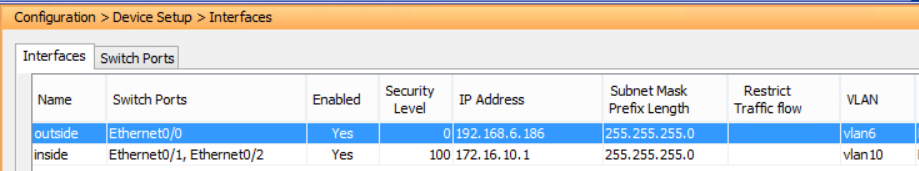
\includegraphics[width=16cm]{Cisco/interfaces.png}
	\caption{Adressage des interfaces}
	\label{fig:ifCisco}
\end{figure}

\subsection{Configuration de l'ASA}
Toute la gestion des connexions et des règles de pare-feu se fait via le même interface graphique, à savoir l'ASDM\footnote{Adaptive Security Device Manager}.
L'ASDM est à installer sur une machine cliente, qui possède Java.

\subsubsection{Gestion des accès}
L'authentification est vérifiée par l'Active Directory. 
Dans ce cas-ci, la configuration est moins simple, vu qu'il faut connaitre les attributs LDAP pour aller chercher dans les OU les utilisateurs et l'administrateur (voir Fig.\ref{fig:authCisco}p.\pageref{fig:authCisco}).
\begin{figure}[ht]
	\centering
	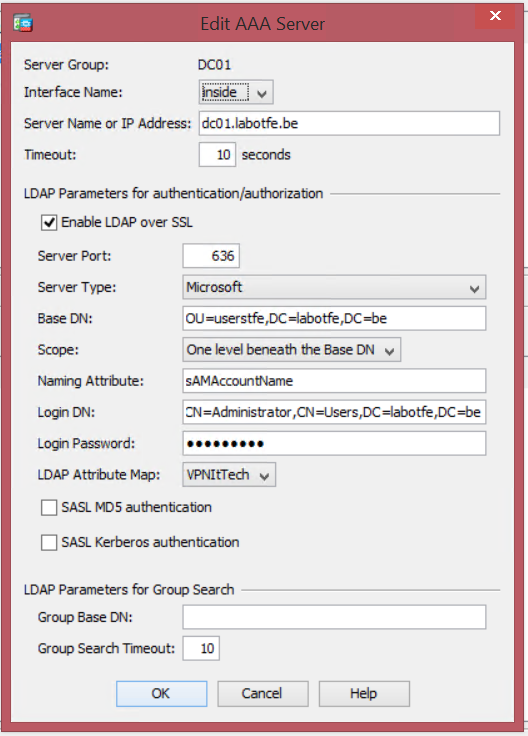
\includegraphics{Cisco/AAA-Ldap.png}
	\caption{Configuration de l'authentification des utilisateurs}
	\label{fig:authCisco}
\end{figure}

\subsubsection{VPN}
Tout d'abord, il faut créer le pool d'adresse pour les clients VPN.
En plus, il est intéressant d'associer des objets aux différents éléments de l'infrastructure pour faciliter la configuration (voir Fig.\ref{fig:objectCisco} p.\pageref{fig:objectCisco}).
\begin{figure}[ht]
	\centering
	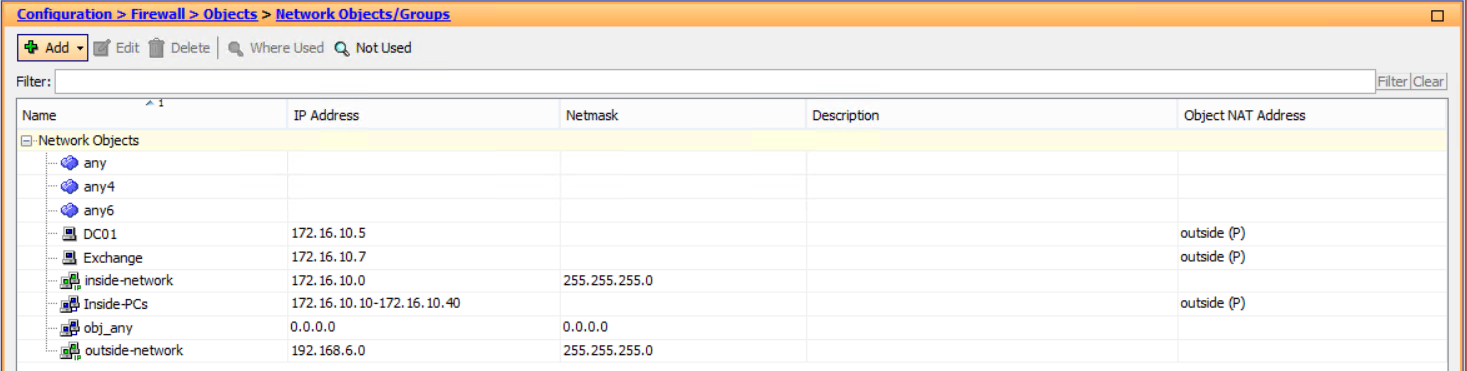
\includegraphics[width=16cm]{Cisco/objects.png}
	\caption{Configuration des objets}
	\label{fig:objectCisco}
\end{figure}

Ensuite, il faut initialiser le "Group Policy".
Ce groupe permet l'attribution des adresses, et aussi de plein de propriétés issues des groupes par défaut, car il hérite par défaut des propriétés des ces groupes. 
Comme on peut le voir sur la Fig.\ref{fig:gpCisco} p.\pageref{fig:gpCisco}, mon groupe \textit{VPNAccess} hérite de deux éléments, par contre pour l'adressage, il va chercher le pool que j'ai défini. 
\begin{figure}[ht]
	\centering
	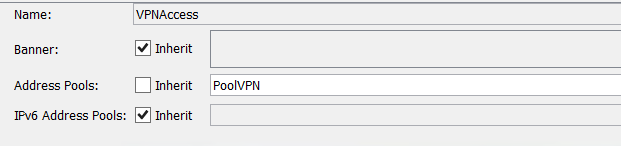
\includegraphics{Cisco/GroupPoliciesVPN.png}
	\caption{Configuration du groupe \textit{VPNAccess}}
	\label{fig:gpCisco}
\end{figure}

Finalement, il reste à configurer le profil de connexion voir Fig.\ref{fig:cpCisco} p.\pageref{fig:cpCisco}.
Il permet de définir le mode d'authentification, et le groupe à associer aux clients.
Particularité, il faut préciser le pool d'adresse même si il est contenu dans le groupe.
\begin{figure}[ht]
	\centering
	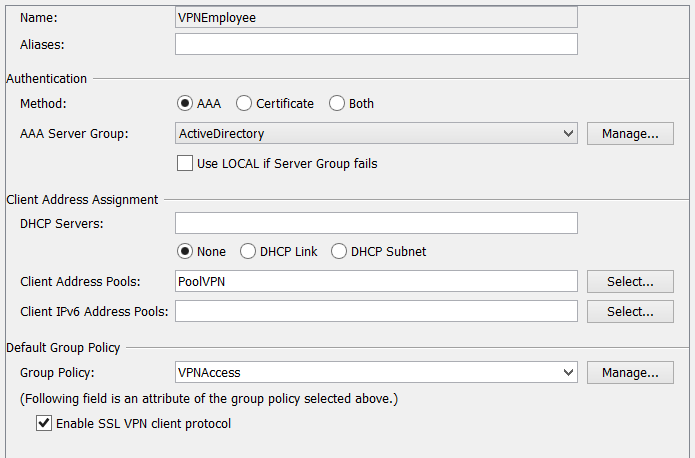
\includegraphics{Cisco/ConnectionProfile.png}
	\caption{Configuration du profil de connexion}
	\label{fig:cpCisco}
\end{figure} 
